% Pedagogical Theory Illustration Primer (Companion to Paper v3)
% Build: latexmk -pdf -interaction=nonstopmode main.tex
\ifdefined\pdftexversion\pdfoutput=1\fi
\documentclass[11pt]{article}

\usepackage[utf8]{inputenc}
\usepackage[T1]{fontenc}
\usepackage[margin=1in, top=1.08in, bottom=0.82in]{geometry}
\setlength{\skip\footins}{26pt}
\usepackage{amsmath, amssymb, amsfonts, mathtools}
\usepackage{graphicx}
\usepackage{booktabs}
\usepackage{multirow}
\usepackage{array}
\usepackage{enumitem}
\usepackage{microtype}
\usepackage{nicefrac}
\usepackage{pifont}
\usepackage[table]{xcolor}
\usepackage[authoryear, sort&compress, round]{natbib}
\PassOptionsToPackage{hyphens}{url}
\usepackage{xurl}
\usepackage[colorlinks, linktoc=page]{hyperref}
\usepackage[nameinlink, capitalize]{cleveref}
\usepackage[palantir]{paperstyle}

\crefname{equation}{}{}
\crefformat{section}{\S#2#1#3}
\crefname{figure}{Figure}{Figures}
\Crefname{figure}{Figure}{Figures}
\captionsetup[figure]{width=0.95\textwidth}
\hypersetup{hypertexnames=false}
\setlength{\headsep}{15pt}

% Consistent colors & callout boxes
\definecolor{colWT}{HTML}{1B4F9C}
\definecolor{colOD}{HTML}{0E7C7B}
\definecolor{colNull}{HTML}{C87D20}
\definecolor{colBad}{HTML}{B83B2A}
\definecolor{colGood}{HTML}{1F7A54}
\definecolor{rowtint}{HTML}{F2F6FC}

\newtcolorbox[auto counter]{toybox}[1][]{%
  enhanced, breakable, lines before break=6, before skip=9pt, after skip=9pt,
  colback=colNull!7!white, colframe=colNull!42!white, boxrule=0.65pt,
  arc=7pt, outer arc=7pt, left=12pt, right=12pt, top=8pt, bottom=8pt,
  coltext=pageink,
  before upper={\noindent{\pagesfsb\color{colNull}Worked $2\times 2$ Example~\thetcbcounter}\ifblank{#1}{}{\enspace\textbf{#1.}}\par\smallskip},
}

\newtcolorbox{plainquestion}[1][]{%
  enhanced, unbreakable, before skip=8pt, after skip=8pt,
  colback=colOD!7!white, colframe=colOD!38!white, boxrule=0.6pt,
  arc=7pt, outer arc=7pt, left=12pt, right=12pt, top=7pt, bottom=7pt,
  coltext=pageink,
  before upper={\noindent{\pagesfsb\color{colOD}Intuition Check}\ifblank{#1}{}{\enspace\textbf{--- #1}}\par\smallskip},
}

\pagestyle{paper}
\papershorttitle{Visual Theory Primer: Understanding Rotation \& Eigenvectors in Output-Normalized Muon}
\graphicspath{{figs/}}
\urlstyle{tt}
\interfootnotelinepenalty=10000

\renewcommand{\topfraction}{0.88}
\renewcommand{\bottomfraction}{0.82}
\renewcommand{\textfraction}{0.08}
\renewcommand{\floatpagefraction}{0.80}

% Notation macros matching Paper v3
\newcommand{\Tr}{{\mathsf{T}}}
\newcommand{\Nten}{\mathcal{N}_{10}}
\newcommand{\unitrms}{\operatorname{unitRMS}}
\newcommand{\tr}{\operatorname{tr}}
\newcommand{\Diag}{\operatorname{Diag}}
\newcommand{\diag}{\operatorname{diag}}
\newcommand{\polar}{\operatorname{polar}}
\newcommand{\E}{\mathbb{E}}
\newcommand{\R}{\mathbb{R}}
\newcommand{\dm}{d_{\mathrm{model}}}
\newcommand{\dff}{d_{\mathrm{ff}}}
\newcommand{\mname}[1]{#1}

\title{Understanding ``Rotation'' and Eigenvector Geometry in Output-Normalized Muon: An Intuitive Visual Guide}
\author{Companion Theory Illustration Paper}
\paperaffiliations{Self-Contained Pedagogical Primer for \emph{Where Output-Cotangent Preconditioning Matters in Muon-Type Optimizers}}

\begin{document}

\maketitle

\begin{abstract}
Modern matrix optimizers such as \mname{Muon}, \mname{MuonT}, and our proposed \mname{WT-MLP-Lag} are often analyzed using dense mathematical language---``backpropagated cotangents,'' ``rotational anisotropy,'' ``Stiefel-tangent rotations,'' ``Haar eigenvector delocalization,'' and ``Dual Procrustes alignment.''
If you do not work daily in matrix-manifold or spectral analysis, those phrases can obscure a remarkably simple, visual chain of cause and effect.

This standalone primer rebuilds the entire theory of output-side normalization from the ground up, assuming \textbf{only basic linear algebra} (matrix multiplication, $90^\circ$ perpendicular vectors, and ellipses in 2D).
Every concept is introduced first through a concrete 2D picture and a hand-checkable $2\times 2$ numerical example before connecting to real \texttt{130M} and \texttt{520M} Transformer measurements.
Specifically, we answer three core questions step by step:
\textbf{(1)~What ``rotation'' actually means}---and why simple per-neuron scaling (like Adam or diagonal \mname{OD-All}) becomes completely blind whenever error clouds tilt at an angle;
\textbf{(2)~Why normalizing outputs changes the singular/eigenvector axes}---solving the apparent paradox of why \mname{Muon}'s polar orthogonalization does \emph{not} erase left-side scaling; and
\textbf{(3)~Why the rotated axis system trains better}---showing how inner fair-voting ($-1/2$), outer canyon-wall damping ($-1/8$), and calmer 20-step momentum work together without inflating the learning rate.
\end{abstract}

% ===========================================================================
\section{The Whole Story in Plain English (Five Connected Steps)}
\label{sec:big_picture}
% ===========================================================================

Before writing a single matrix equation, let us trace the complete logic of the main paper in five everyday steps (\Cref{fig:roadmap}). Every technical theorem later in this guide is simply a precise version of one of these five boxes:

\begin{figure}[t]
  \centering
  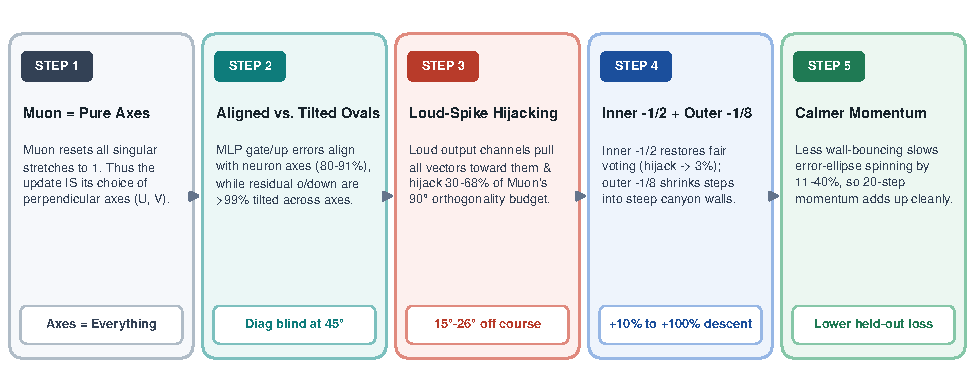
\includegraphics[width=\textwidth]{fig1_logic_roadmap.pdf}
  \caption{\textbf{The five-step cause-and-effect chain behind output-side normalization (\mname{WT-MLP-Lag}).} Reading from left to right answers \emph{why axes matter in \mname{Muon}} (Step~1), \emph{what ``rotation'' means} (Step~2), \emph{why normalization changes the axes instead of cancelling out} (Step~3), and \emph{why the new axes train better both immediately and over hundreds of steps} (Steps~4--5).}
  \label{fig:roadmap}
\end{figure}

\begin{enumerate}[leftmargin=1.65em, itemsep=4pt, topsep=4pt]
  \item \textbf{Step 1 --- Why axes are everything in \mname{Muon}:}
  In standard gradient descent, a weight layer's gradient matrix usually stretches a tiny handful of ``loud'' directions strongly while barely moving hundreds of quieter feature directions.
  \mname{Muon}~\citep{jordan2024muon} fixes this by applying a \emph{polar step} that resets \textbf{every perpendicular stretch factor to $1$}.
  Once all stretch factors are forced to $1$, there are no stretch factors left to tune inside \mname{Muon}: \emph{the entire optimization step IS its choice of perpendicular input and output coordinate axes!}

  \item \textbf{Step 2 --- What ``rotation'' means (aligned ovals vs.\ tilted ovals):}
  As errors travel backward through a Transformer, some output directions fluctuate much more wildly than others---forming a stretched \textbf{oval (ellipse)} rather than a round circle.
  \begin{itemize}[leftmargin=1.4em, itemsep=1.5pt, topsep=2pt]
    \item Behind the MLP's elementwise SwiGLU gate (\texttt{gate}, \texttt{up}), that oval lines up neatly with the individual neuron axes ($78\%\text{--}91\%$ axis-aligned). Simple per-neuron rescaling fixes it cheaply.
    \item On the shared residual highway (\texttt{o}, \texttt{down}), dozens of layers mix all neurons together, \textbf{tilting the oval diagonally across coordinates} ($>99\%$ tilted). When an oval is tilted at $45^\circ$, its shadow on Neuron~1 and its shadow on Neuron~2 have the \emph{exact same width}---making per-neuron diagonal scalers completely blind! To fix a tilted oval, you \emph{must} rotate into its tilted axes (its eigenvectors).
  \end{itemize}

  \item \textbf{Step 3 --- Why normalizing outputs changes \mname{Muon}'s axes (``Loud-Spike Hijacking''):}
  At first glance, multiplying rows by a normalizer \emph{before} \mname{Muon} seems pointless: if \mname{Muon} resets all singular stretches back to $1$ anyway, shouldn't row scaling get undone?
  \textbf{No!} When one output channel is $10\times$ louder in error noise, it acts like a magnet that pulls \emph{all} gradient vectors toward that loud axis.
  When \mname{Muon} subsequently forces those vectors back to $90^\circ$ perpendicularity, the loudest vector hogs the loud axis and \textbf{shoves quieter feature vectors $15^\circ\text{--}26^\circ$ off course}.
  Normalizing output variance by $B^{-1/2}$ \emph{before} \mname{Muon} turns down the megaphone before the $90^\circ$ vote happens.

  \item \textbf{Step 4 --- Why the new axis system steps downhill more safely (Inner $-1/2$ + Outer $-1/8$):}
  Our method applies two output adjustments that act at \textbf{$90^\circ$ right angles} to each other:
  \begin{itemize}[leftmargin=1.4em, itemsep=1.5pt, topsep=2pt]
    \item \textbf{Inner $B^{-1/2}$ (inside \mname{Muon} --- ``Fair Compass''):} Eliminates loud-channel hijacking (dropping top-error hijacking from $30\%\text{--}68\%$ down to the $3.1\%$ random-chance floor) so $69\%\text{--}82\%$ of quieter features align better with their true gradient signal.
    \item \textbf{Outer $B^{-1/8}$ (outside \mname{Muon} --- ``Canyon Cushion''):} After \mname{Muon} gives every axis equal step length $1$, stepping full-speed into a $40\times$ steeper canyon wall causes overshoot. Gently shrinking steps into steep walls with $B^{-1/8}$ (normalized to keep total step size unchanged!) cuts canyon curvature shock by up to $55\%$ and boosts downhill efficiency by $+10\%\text{--}100\%$, without blowing up minibatch noise like steeper $-1/4$ exponents (\mname{GO-MUON}).
  \end{itemize}

  \item \textbf{Step 5 --- Why momentum snowballs over hundreds of steps:}
  \mname{Muon} averages roughly $20$ past steps via Nesterov momentum ($\mu = 0.95$).
  When an optimizer repeatedly bounces off steep error canyon walls, the network's internal error ovals lurch and spin rapidly, causing old momentum vectors to fight new gradients.
  Because \mname{WT-MLP-Lag} stops hitting those walls, error ovals spin \textbf{$11\%\text{--}40\%$ slower} across all seven layer types, letting 20-step momentum add up smoothly toward lower validation loss.
\end{enumerate}

% ===========================================================================
\section{Building Blocks from Zero: Matrices, Ellipses, and Muon}
\label{sec:primer}
% ===========================================================================

Let us now build the three simple mathematical pictures we need, stripping away all unnecessary jargon.

\subsection{Two Vectors Meet at Every Linear Layer: Input \texorpdfstring{$x$}{x} and Backward Error \texorpdfstring{$\delta$}{delta}}
\label{sec:x_and_delta}

Consider any linear weight matrix $W \in \R^{m \times n}$ inside a Transformer (such as Query $W_q$, Output $W_o$, or MLP $W_{\mathrm{down}}$). For each token in a training batch:
\begin{enumerate}[leftmargin=1.6em, itemsep=2pt, topsep=2pt]
  \item \textbf{Forward pass ($y = W x$):} An input vector $x \in \R^n$ enters from the right (matching the $n$ \emph{columns} of $W$) and produces an output vector $y \in \R^m$ on the left (matching the $m$ \emph{rows} of $W$).
  \item \textbf{Backward pass ($\delta = \partial\mathcal{L}/\partial y$):} Backpropagation sends an \textbf{output error vector} $\delta \in \R^m$ arriving at $y$.
  \emph{Jargon alert:} Optimization papers call $\delta$ the \textbf{output cotangent} simply because $x$ moves forward (a ``tangent'' vector) while derivatives $\partial\mathcal{L}/\partial y$ move backward (a ``cotangent'' vector). Whenever you read \emph{cotangent $\delta$} in the main paper, read \textbf{``the layer's backpropagated output error vector.''}
\end{enumerate}

How does weight entry $W_{ab}$ (row $a$, column $b$) get its gradient? By the chain rule, changing $W_{ab}$ nudges output $y_a$ in proportion to input $x_b$, which changes the loss by $\delta_a x_b$. Stacking all rows $a$ and columns $b$ into a matrix and summing over $N$ tokens in the batch gives the weight gradient:
\begin{equation}
  G = \sum_{j=1}^{N} \delta_j x_j^{\Tr} \;\in\; \R^{m \times n}.
  \label{eq:grad_outer}
\end{equation}
Notice the clean two-sided symmetry of \eqref{eq:grad_outer} (\Cref{fig:primer}c): \textbf{output errors $\delta$ live on the left (rows of $G$)}, while \textbf{input activations $x$ live on the right (columns of $G$)}.

To measure how stretched or tilted the cloud of inputs $x$ and the cloud of backward errors $\delta$ are, we track their running average outer products (\textbf{second-moment matrices}):
\begin{equation}
  C = \E\!\left[x x^{\Tr}\right] \in \R^{n \times n} \quad (\text{input cloud shape}),
  \qquad
  B = \E\!\left[\delta \delta^{\Tr}\right] \in \R^{m \times m} \quad (\text{error cloud shape}).
  \label{eq:moments_simple}
\end{equation}

\begin{figure}[t]
  \centering
  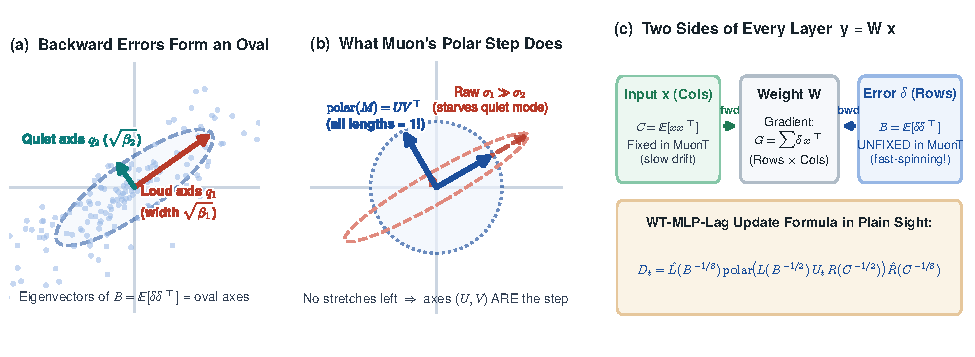
\includegraphics[width=\textwidth]{fig2_svd_muon_primer.pdf}
  \caption{\textbf{Visual primer on eigenvectors, singular vectors, and \mname{Muon}.}
  \textbf{(a)} Plotting backward error vectors $\delta$ over a batch forms an ellipse; the eigenvectors $q_1, q_2$ of $B = \E[\delta\delta^{\Tr}]$ are simply the ellipse's perpendicular principal axes, and $\sqrt{\beta_1}, \sqrt{\beta_2}$ are its widths.
  \textbf{(b)} A raw momentum matrix $M = U\Sigma V^{\Tr}$ stretches one axis vastly more than another ($\sigma_1 \gg \sigma_2$, dashed red), starving quiet features; \mname{Muon}'s polar step $\polar(M) = U V^{\Tr}$ resets all stretches to $1$ (solid blue circle), making the choice of axes $(U, V)$ the entire update.
  \textbf{(c)} Because $G = \sum \delta x^{\Tr}$, input-only \mname{MuonT} fixes the right-hand input ellipse $C$ while leaving the left-hand backward error ellipse $B$ unfixed.}
  \label{fig:primer}
\end{figure}

\subsection{Eigenvectors vs.\ Singular Vectors in One Picture}
\label{sec:eig_vs_svd}

Beginners often ask: \emph{what is the intuitive difference between eigenvectors and singular vectors?} Both describe perpendicular axes of an ellipse---just for two different kinds of matrices:

\begin{itemize}[leftmargin=1.5em, itemsep=3pt, topsep=3pt]
  \item \textbf{Eigenvectors (for a square symmetric cloud matrix like $B = \E[\delta\delta^{\Tr}]$):}
  Plot thousands of backward error vectors $\delta_j$ as dots in space (\Cref{fig:primer}a). If errors were equally strong and uncorrelated in every direction (\textbf{isotropic}), the cloud would form a round sphere ($B \propto I$).
  In reality, errors form an elongated \textbf{ellipse} (\textbf{anisotropic} = ``not round'').
  Every symmetric matrix $B$ factors as
  \begin{equation}
    B = Q \Lambda Q^{\Tr} = \sum_{i=1}^{m} \beta_i\, q_i q_i^{\Tr},
    \label{eq:eig}
  \end{equation}
  where the \textbf{eigenvectors} $q_1, \dots, q_m$ (columns of orthogonal matrix $Q$, $Q^{\Tr}Q = I$) are literally \emph{the perpendicular compass axes of the ellipse}, and the \textbf{eigenvalues} $\beta_1 \ge \dots \ge \beta_m \ge 0$ are \emph{the squared widths (variances) along each axis}.

  \item \textbf{Singular Value Decomposition / SVD (for a rectangular update matrix $M \in \R^{m \times n}$):}
  An update or momentum matrix $M$ maps $n$-dimensional inputs to $m$-dimensional outputs, so its input space and output space are different.
  Remarkably, \emph{any} matrix $M$ acts in three elementary steps:
  \begin{equation}
    M = U \Sigma V^{\Tr} = \sum_{i=1}^{r} \sigma_i\, u_i v_i^{\Tr},
    \label{eq:svd}
  \end{equation}
  meaning: \textbf{(1)}~read components along perpendicular \emph{input axes} $v_i$ (right singular vectors), \textbf{(2)}~stretch axis $i$ by \emph{singular value} $\sigma_i \ge 0$, and \textbf{(3)}~place the result along perpendicular \emph{output axes} $u_i$ (left singular vectors).
\end{itemize}

\subsection{What Muon Actually Does --- And Why Axes Are the Whole Game}
\label{sec:what_muon_does}

Why not just update weights with raw Nesterov momentum $U_t$ ($W_{t+1} = W_t - \eta U_t$)?
In Transformer training, the top singular value $\sigma_1$ of $U_t$ is routinely $10\times\text{--}50\times$ larger than bulk singular values $\sigma_k$ (\Cref{fig:primer}b, dashed red ellipse).
If you pick a learning rate $\eta$ small enough not to explode along $\sigma_1$, then $80\%+$ of the layer's feature directions barely move at all!

\mname{Muon}~\citep{jordan2024muon} solves this feature starvation with a single bold operation called \textbf{polar orthogonalization}: keep the singular vector axes $(U, V)$ intact, and replace \emph{every} singular value $\sigma_i$ with $1$:
\begin{equation}
  \polar(M) \;\triangleq\; U V^{\Tr} \qquad \text{when } M = U \Sigma V^{\Tr}.
  \label{eq:polar_def}
\end{equation}
Computing an exact SVD on GPUs is slow, so \mname{Muon} approximates $\polar(M)$ using 10 fast matrix-multiply iterations of a polynomial called \textbf{Newton--Schulz} (written $\Nten(M)$ in the main paper), which pushes every singular value $\sigma_i \to 1$ without ever forming $U$ or $V$ explicitly.

\begin{keyfinding}[Why Axes Matter So Much in Muon]
Because $\polar(M) = U V^{\Tr}$ erases unequal singular stretches ($\Sigma \to I$), \textbf{two \mname{Muon}-style updates with equal step norm differ purely by which perpendicular axes $(U, V)$ they pair together!}
Input-whitened \mname{MuonT}~\citep{mohamadi2026toner} fixes distortion in the right-hand input axes $V$ using $C^{-1/2}$, but leaves the left-hand output axes $U$ at the mercy of raw backward error spikes $B$ (\Cref{fig:primer}c).
\end{keyfinding}

To make reading the main paper effortless, \Cref{tab:decoder} translates every technical phrase in \texttt{paper\_v3} into the concrete visual language we use throughout this guide.

\begin{table}[t]
  \centering
  \caption{\textbf{The Plain-English Jargon Decoder.} Every specialized term in the main paper maps to a concrete 2D geometric picture.}
  \label{tab:decoder}
  \vspace{2pt}
  \footnotesize
  \renewcommand{\arraystretch}{1.22}
  \begin{tabular}{@{}>{\raggedright\arraybackslash}p{0.31\textwidth}>{\raggedright\arraybackslash}p{0.65\textwidth}@{}}
    \toprule
    \textbf{Term in Main Paper (\texttt{paper\_v3})} & \textbf{What It Actually Means in Plain English} \\
    \midrule
    \textbf{Output cotangent $\delta_t$} & Simply the backpropagated error vector $\partial\mathcal{L}/\partial y_t$ arriving at the output of linear layer $y = W x$. \\
    \textbf{Second moment $B_t = \E[\delta\delta^{\Tr}]$} & Average shape of the backward error cloud: its eigenvectors are the error oval's axes; its eigenvalues $\beta_i$ are the squared widths along each axis. \\
    \textbf{Coordinate vs.\ rotational anisotropy} & \emph{Coordinate}: oval aligns with neuron axes ($B_{11} \neq B_{22}$, off-diagonals $=0$). \emph{Rotational}: oval is tilted across neurons ($B_{11} \approx B_{22}$, off-diagonals $\neq 0$). \\
    \textbf{Stiefel manifold $\{O : O O^{\Tr}=I_m\}$} & Just the set of matrices whose $m$ rows are unit-length and $90^\circ$ perpendicular (in 2D, simply the unit circle of rotation matrices!). \\
    \textbf{Stiefel-tangent vs.\ normal step} & \emph{Tangent} (inner $L$): rotates the axes \emph{along} the unit circle while keeping lengths $=1$. \emph{Normal} (outer $\hat{L}$): stretches/shrinks step lengths \emph{perpendicular} to the circle. \\
    \textbf{Dual Weighted Procrustes / CCA} & Choosing $90^\circ$ perpendicular update axes by \emph{fair correlation} between inputs and errors ($L=B^{-1/2}$), instead of letting the loudest error channel bully the vote. \\
    \textbf{Haar delocalization ($\mathrm{IPR} \approx 3.0$)} & Residual-stream error axes point in thoroughly mixed directions across all $\dm$ neurons, averaging out per-neuron variance differences as $2/(\dm+2)$. \\
    \textbf{Kronecker shock $\mathcal{Q}_{B,C}$ \& $\Phi_{B,C}$} & $\mathcal{Q}_{B,C}$ measures how hard a unit step slams into steep canyon walls; $\Phi_{B,C} = \text{slope}^2 / \mathcal{Q}_{B,C}$ measures net downhill progress per unit canyon curvature. \\
    \textbf{Subspace Grassmann drift ($\mathrm{Drift}_{16}$)} & How fast the top 16 axes of the error oval spin over 250 training steps ($0 =$ frozen axes; $1 =$ spun into a completely perpendicular subspace). \\
    \bottomrule
  \end{tabular}
\end{table}

% ===========================================================================
\section{What ``Rotation'' Means --- And Why Diagonal Scaling Goes Blind}
\label{sec:rotation_meaning}
% ===========================================================================

A common source of confusion when reading optimization papers is that the word \textbf{``rotation''} appears in three different places. Keeping them distinct immediately clears the fog:
\begin{enumerate}[leftmargin=1.6em, itemsep=2pt, topsep=2pt]
  \item \textbf{Static tilt of the error oval ($B_t$):} The principal axes (eigenvectors) of $B_t$ are tilted away from the standard neuron axes $(1,0,\dots,0)$ (\Cref{fig:tilted}b).
  \item \textbf{Spinning of that oval over training time ($\mathrm{Drift}_{16}$):} From step $t$ to step $t+250$, those tilted axes themselves slowly (or rapidly!) spin as weights evolve.
  \item \textbf{Steering of the weight update ($\theta(D_{\mathrm{WT}}, D_{\mathrm{MuonT}}) \approx 15^\circ\text{--}25^\circ$):} Adding output normalization changes \emph{which direction} the weight matrix steps in, without increasing step length.
\end{enumerate}

Let us start with Meaning~1, because it explains \textbf{why popular per-neuron optimizers (like Adam or purely diagonal \mname{OD-All}) completely miss residual-stream geometry}.

\begin{toybox}[Why a $45^\circ$-Tilted Error Oval Makes Diagonal Scaling 100\% Blind]
Suppose a 2-neuron layer experiences a sharp $49:1$ error variance imbalance between its steepest error axis ($\beta_1 = 1.96 = 1.4^2$) and its flattest error axis ($\beta_2 = 0.04 = 0.2^2$, a $7\times$ width stretch). Notice that the average variance is $\frac{1}{2}(1.96 + 0.04) = 1.00$. Compare two orientations of \textbf{the exact same $7:1$ oval} (\Cref{fig:tilted}a vs.\ \Cref{fig:tilted}b):

\textbf{Case A --- Axis-Aligned Oval (like \texttt{out:gate} and \texttt{out:up}):}
\[
  B_{\mathrm{aligned}} = \begin{pmatrix} 1.96 & 0 \\ 0 & 0.04 \end{pmatrix}.
\]
Here Neuron~1 fluctuates wildly ($B_{11}=1.96$) and Neuron~2 barely fluctuates ($B_{22}=0.04$). A cheap per-neuron diagonal scaler looks \emph{only} at the diagonal $(1.96,\, 0.04)$, divides Neuron~1 by $\sqrt{1.96}=1.4$ and divides Neuron~2 by $\sqrt{0.04}=0.2$, and \textbf{turns the oval into a perfect unit circle!}

\smallskip
\textbf{Case B --- The Exact Same Oval Tilted by $45^\circ$ (like \texttt{out:o} and \texttt{out:down}):}
Rotate $B_{\mathrm{aligned}}$ by $45^\circ$ using $Q_{45^\circ} = \frac{1}{\sqrt{2}}\begin{psmallmatrix} 1 & -1 \\ 1 & 1 \end{psmallmatrix}$:
\[
  B_{\mathrm{tilted}}
  = Q_{45^\circ}\begin{pmatrix} 1.96 & 0 \\ 0 & 0.04 \end{pmatrix} Q_{45^\circ}^{\Tr}
  = \begin{pmatrix} \mathbf{1.00} & 0.96 \\ 0.96 & \mathbf{1.00} \end{pmatrix}.
\]
\textbf{Look at the diagonal entries:} $B_{11} = \mathbf{1.00}$ and $B_{22} = \mathbf{1.00}$!
Because the $+45^\circ$ canyon affects Neuron~1 and Neuron~2 equally ($\delta_1 \approx +\delta_2$), both neurons cast the \emph{exact same shadow width} on the $x$-axis and $y$-axis (\Cref{fig:tilted}b, red bars).
A diagonal preconditioner inspects only $(B_{11}, B_{22}) = (1.00, 1.00)$ and concludes: \emph{``Every neuron already has variance $1.00$! Do nothing ($\Diag(B_{\mathrm{tilted}})^{-1/2} = I_2$)!''}
Only the dense matrix inverse square root
\[
  B_{\mathrm{tilted}}^{-1/2}
  = Q_{45^\circ}\begin{pmatrix} 1/1.4 & 0 \\ 0 & 1/0.2 \end{pmatrix} Q_{45^\circ}^{\Tr}
  = \begin{pmatrix} 2.857 & -2.143 \\ -2.143 & 2.857 \end{pmatrix}
\]
rotates by $45^\circ$ into the oval's true eigenvectors $(1,1)/\sqrt{2}$ and $(-1,1)/\sqrt{2}$, shrinks the $+45^\circ$ canyon by $1.4\times$, and stretches the $-45^\circ$ valley by $5\times$!
\end{toybox}

\begin{figure}[t]
  \centering
  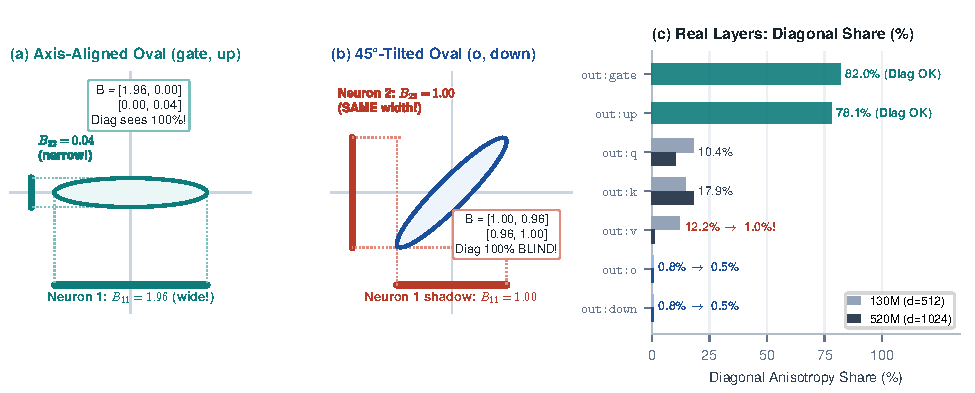
\includegraphics[width=\textwidth]{fig3_tilted_vs_aligned.pdf}
  \caption{\textbf{Axis-aligned vs.\ tilted error ovals---from 2D geometry to real \texttt{130M} and \texttt{520M} Transformers.}
  \textbf{(a)} When the error oval aligns with neuron axes ($B_{\mathrm{aligned}}$), shadows on Neuron~1 and Neuron~2 differ sharply ($1.96$ vs.\ $0.04$), so 1D diagonal scaling sees $100\%$ of the distortion.
  \textbf{(b)} Tilting the exact same oval by $45^\circ$ ($B_{\mathrm{tilted}}$) makes the Neuron~1 and Neuron~2 shadows \emph{identical} ($B_{11}=B_{22}=1.00$), leaving diagonal scaling $100\%$ blind!
  \textbf{(c)} Real Transformer output moments mirror both extremes: SwiGLU-gated \texttt{out:gate, up} sit at $78\%\text{--}82\%$ diagonal, whereas residual-stream \texttt{out:o, down} sit below $1\%$ diagonal at \texttt{130M} ($d=512$) and shrink further to $0.50\%$ at \texttt{520M} ($d=1{,}024$)---with \texttt{out:v} collapsing $12\times$ from $12.2\% \to 1.0\%$.}
  \label{fig:tilted}
\end{figure}

\subsection{Why Transformers Produce Both Extremes (SwiGLU Gate vs.\ Residual Mixing Bowl)}
\label{sec:why_transformer_splits}

Why do some layers in a Transformer behave like Case~A while others behave like Case~B (\Cref{fig:tilted}c)? The architecture itself creates both regimes:

\paragraph{1. Why \texttt{out:gate} and \texttt{out:up} are axis-aligned (The SwiGLU Scrambler).}
Inside an MLP block, \texttt{gate} and \texttt{up} expand $\dm$ dimensions to $\dff = 4\dm$ neurons and immediately multiply element-by-element: $z_i = \operatorname{SiLU}(y_{\mathrm{gate},i})\cdot y_{\mathrm{up},i}$.
During backpropagation, each neuron $i$'s error gets multiplied by its own forward activation gate.
Because neuron $i$'s forward gate in layer $\ell$ has almost nothing to do with cross-channel prediction errors coming down from upper layers on neuron $j \neq i$, off-diagonal correlations $B_{ij}$ cancel out right down to random batch-sampling noise ($\approx 0.005$).
Meanwhile, active vs.\ quiet neurons develop large per-neuron variance differences along the diagonal ($78\%\text{--}91\%$ axis-aligned!).
\emph{Payoff:} Replacing slow $O(\dff^3)$ matrix eigendecompositions on \texttt{gate} and \texttt{up} with cheap $O(\dff)$ diagonal scaling saves \textbf{$96.2\%$ of output eigendecomposition compute} with \emph{zero} accuracy loss!

\paragraph{2. Why \texttt{out:o} and \texttt{out:down} are tilted---and why wider models blind diagonal scaling even further (The Residual Mixing Bowl).}
By contrast, $W_o$ (end of Attention) and $W_{\mathrm{down}}$ (end of MLP) add their outputs directly into the \textbf{shared residual stream} with no elementwise gate in the way.
As backward errors travel down $(L-\ell)$ Transformer blocks, they pass through dozens of dense attention and MLP matrices that thoroughly stir all $\dm$ coordinates together---like stirring paint in a bowl.

In the main paper, we test how thoroughly mixed an eigenvector $q_k = (q_{k1},\dots,q_{kd})^{\Tr}$ is using a simple spread score called the \textbf{Inverse Participation Ratio}, $\mathrm{IPR}(q_k) = d\sum_{i=1}^{d} q_{ki}^4$:
\begin{itemize}[leftmargin=1.5em, itemsep=1.5pt, topsep=2pt]
  \item If an eigenvector points along a \emph{single} neuron axis $(1,0,\dots,0)$, then $\mathrm{IPR} = d$ ($=512$ or $1{,}024$).
  \item If an eigenvector points in a \emph{completely mixed random direction} (called ``Haar-random'' in math), every coordinate carries $\approx \pm 1/\sqrt{d}$ weight and $\mathrm{IPR} \approx \mathbf{3.00}$.
\end{itemize}
In real \texttt{130M} and \texttt{520M} checkpoints, \texttt{out:o} and \texttt{out:down} have median $\mathrm{IPR} = \mathbf{3.01}$!
Because every neuron $i$ averages all $\dm$ tilted ellipse axes roughly equally ($B_{ii} = \sum_{k=1}^{\dm} Q_{ik}^2 \beta_k \approx \bar{\beta}$), the \textbf{Law of Large Numbers} averages away neuron-to-neuron variance differences in proportion to $1/\dm$:
\begin{equation}
  \text{Diagonal Share of } B \;\approx\; \frac{2}{\dm + 2}
  \quad\Longrightarrow\quad
  \begin{cases}
    0.78\% & \text{measured at \texttt{130M} } (\dm = 512), \\
    \mathbf{0.50\%} & \text{measured at \texttt{520M} } (\dm = 1{,}024).
  \end{cases}
  \label{eq:mixing_bowl}
\end{equation}
Even though the tilted residual error oval is $>40\times$ steeper in some directions than others, $>99.5\%$ of that geometry is invisible on the diagonal at $\dm=1{,}024$! That is why purely diagonal output scaling (\mname{OD-All}) helps slightly at \texttt{130M} but loses its margin when scaling to \texttt{520M}.

% ===========================================================================
\section{Why Normalization Changes the Axes (Why Polar Doesn't Undo It)}
\label{sec:hijacking}
% ===========================================================================

Now we arrive at the sharpest conceptual puzzle in the entire story:

\begin{plainquestion}[The Cancellation Paradox]
In \mname{WT-MLP-Lag}, we multiply the input-whitened momentum $Z_0 = U_t R_t$ on the left by $L = B^{-1/2}$ \emph{inside} \mname{Muon}'s polar orthogonalizer: $\polar(L Z_0)$.
Wait a second! Since $\polar(\cdot)$ throws away all singular values and resets every singular stretch back to $1$, why doesn't $\polar(L Z_0)$ give the \textbf{exact same orthogonal matrix} as $\polar(Z_0)$?
\end{plainquestion}

The answer is both surprising and wonderfully visual. Let us work out a $2\times 2$ example using \textbf{nothing beyond $\sin\phi$ and $\cos\phi$}!

\subsection{A High-School-Trig Formula for \texorpdfstring{$2\times 2$}{2x2} Polar Orthogonalization}
\label{sec:2x2_trig}

For any $2\times 2$ matrix $A = \begin{psmallmatrix} a & b \\ c & d \end{psmallmatrix}$ with $\det(A) > 0$, $\polar(A)$ is simply the 2D rotation matrix $R(\phi) = \begin{psmallmatrix} \cos\phi & -\sin\phi \\ \sin\phi & \cos\phi \end{psmallmatrix}$ closest to $A$---meaning it maximizes the dot product $\tr(R(\phi)^{\Tr} A) = (a+d)\cos\phi + (c-b)\sin\phi$.
By basic trigonometry, $X\cos\phi + Y\sin\phi$ peaks at the exact angle $\phi$ where
\begin{equation}
  \tan\phi \;=\; \frac{c - b}{a + d}.
  \label{eq:tan_phi}
\end{equation}
Equation~\eqref{eq:tan_phi} lets you compute the exact polar rotation of \emph{any} $2\times 2$ matrix in five seconds by hand! Watch what happens when we plug two matrices into \eqref{eq:tan_phi}:

\begin{toybox}[How a $10\times$ Loud Output Channel Hijacks Polar Axes by $26.2^\circ$]
Suppose the clean, noise-free feature signal $M_{\mathrm{true}}$ wants to update two $90^\circ$-perpendicular directions at $\mathbf{45^\circ}$ and $\mathbf{135^\circ}$ ($P_{\mathrm{ideal}} = R(45^\circ) = \frac{1}{\sqrt{2}}\begin{psmallmatrix} 1 & -1 \\ 1 & 1 \end{psmallmatrix}$).

\textbf{Warmup --- What if both features had EQUAL strength ($\sigma_1 = \sigma_2 = 1$)?}
Suppose we distort Output Row~1 by a $10\times$ loud error multiplier $\Lambda_B^{1/2} = \begin{psmallmatrix} 10 & 0 \\ 0 & 1 \end{psmallmatrix}$:
\begin{align*}
  Z_{\mathrm{equal}}
  &= \begin{pmatrix} 10 & 0 \\ 0 & 1 \end{pmatrix} \frac{1}{\sqrt{2}}\begin{pmatrix} 1 & -1 \\ 1 & 1 \end{pmatrix}
   = \frac{1}{\sqrt{2}}\begin{pmatrix} 10 & -10 \\ 1 & 1 \end{pmatrix}, \\
  \tan\phi &= \frac{1 - (-10)}{10 + 1} = \frac{11}{11} = 1 \quad\Longrightarrow\quad \phi = \mathbf{45.0^\circ}.
\end{align*}
\emph{Aha!} When $\sigma_1 = \sigma_2$, the $10\times$ row stretch \textbf{really does cancel out completely}!

\smallskip
\textbf{Real Life --- Features have UNEQUAL strengths ($\sigma_1 = 2.0$, $\sigma_2 = 0.5$; \Cref{fig:hijacking}a--c):}
In every real neural network gradient, some features have stronger raw signal than others:
\begin{align*}
  M_{\mathrm{true}}
  &= \underbrace{\frac{1}{\sqrt{2}}\begin{pmatrix} 1 & -1 \\ 1 & 1 \end{pmatrix}}_{45^\circ\text{ axes}}
     \underbrace{\begin{pmatrix} 2.0 & 0 \\ 0 & 0.5 \end{pmatrix}}_{\sigma_1=2.0,\;\sigma_2=0.5}
   = \frac{1}{\sqrt{2}}\begin{pmatrix} 2.0 & -0.5 \\ 2.0 & 0.5 \end{pmatrix}, \\
  \tan\phi_{\mathrm{true}} &= \frac{2.0 - (-0.5)}{2.0 + 0.5} = \frac{2.5}{2.5} = 1 \quad\Longrightarrow\quad \phi_{\mathrm{true}} = \mathbf{45.0^\circ}.
\end{align*}
Now let Output Row~1 carry $10\times$ louder error variance ($\Lambda_B^{1/2} = \diag(10, 1)$). Without output normalization (\mname{MuonT}), \mname{Muon} receives:
\[
  Z_0
  = \begin{pmatrix} 10 & 0 \\ 0 & 1 \end{pmatrix} M_{\mathrm{true}}
  = \frac{1}{\sqrt{2}}\begin{pmatrix} \mathbf{20} & \mathbf{-5} \\ 2 & 0.5 \end{pmatrix}.
\]
Plug $Z_0$ into our exact polar angle formula~\eqref{eq:tan_phi}:
\[
  \tan\phi_0 \;=\; \frac{2 - (-5)}{20 + 0.5} \;=\; \frac{7}{20.5} \;\approx\; 0.3415
  \quad\Longrightarrow\quad
  \phi_0 \;=\; \arctan(0.3415) \;=\; \mathbf{18.85^\circ}!
\]
\textbf{What just happened geometrically (\Cref{fig:hijacking}b,c)?}
\begin{enumerate}[leftmargin=1.5em, itemsep=1.5pt, topsep=2pt]
  \item Multiplying horizontal Row~1 by $10$ dragged \emph{both} columns almost flat onto the loud horizontal axis: Column~1 has length $\mathbf{14.2}$ at $5.7^\circ$, and Column~2 has length $\mathbf{3.6}$ at $174.3^\circ$.
  \item Now $\polar(Z_0)$ forces the two columns to be $90^\circ$ apart again while maximizing length-weighted alignment $14.2\cos\theta_1 + 3.6\cos\theta_2$. Because Column~1 is $4\times$ longer, $\polar(Z_0)$ caters to Column~1---letting it hog the loud horizontal axis ($18.85^\circ$) and \textbf{bullying quiet Column~2 off course by $26.15^\circ$} ($108.85^\circ$ instead of $135^\circ$)!
  \item Pre-multiplying by $L = B^{-1/2} = \diag(\nicefrac{1}{10}, 1)$ \emph{before} $\polar(\cdot)$ divides Row~1 back by $10$ ($L Z_0 = M_{\mathrm{true}}$), restoring fair voting and recovering the \textbf{exact $45.0^\circ$ axes}!
\end{enumerate}
\end{toybox}

\begin{figure}[t]
  \centering
  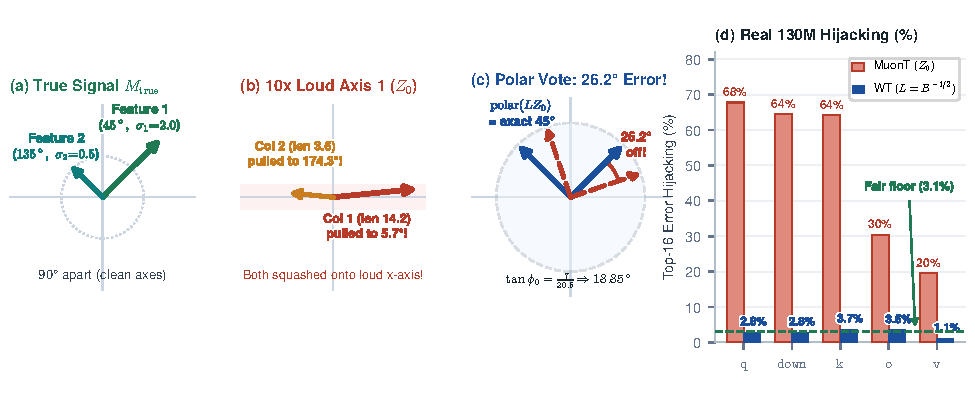
\includegraphics[width=\textwidth]{fig4_hijacking_2x2.pdf}
  \caption{\textbf{Visualizing ``Loud-Channel Hijacking'' inside \mname{Muon}'s polar step---and its cure.}
  \textbf{(a)} Clean feature matrix $M_{\mathrm{true}}$ has perpendicular axes at $45^\circ$ ($\sigma_1=2.0$) and $135^\circ$ ($\sigma_2=0.5$).
  \textbf{(b)} When Output Row~1 is $10\times$ louder in error noise ($Z_0$), both feature vectors get squashed toward the horizontal $x$-axis ($5.7^\circ$ and $174.3^\circ$).
  \textbf{(c)} Forcing $90^\circ$ orthogonality via $\polar(Z_0)$ lets loud Column~1 bully quiet Column~2 off course by $\mathbf{26.2^\circ}$ ($18.85^\circ$, dashed red), whereas inner normalization $\polar(L Z_0)$ restores the exact $45^\circ$ axes (solid blue).
  \textbf{(d)} Across all 32 layers of a real \texttt{130M} Transformer, top-16 noisy error directions hijack $30\%\text{--}68\%$ of \mname{MuonT}'s top-16 pre-polar singular axes (red); applying $L = B^{-1/2}$ drops hijacking right onto the $3.1\%$ fair-chance baseline (blue).}
  \label{fig:hijacking}
\end{figure}

\subsection{Connecting the \texorpdfstring{$2\times 2$}{2x2} Picture to Real Transformers and \texorpdfstring{$\Nten$}{N10}}
\label{sec:hijack_transformer}

In the main paper, Equation~(5) writes the general $m \times n$ version of our $2\times 2$ discovery:
\begin{equation}
  \polar(L Z_0) \;=\; \Omega\,\polar(Z_0),
  \qquad
  \Omega = \polar(L S_0) \in SO(m),
  \label{eq:general_rotation}
\end{equation}
where $S_0 = (Z_0 Z_0^{\Tr})^{1/2}$ encodes the unequal singular stretches of $Z_0$. Whenever $Z_0$ has unequal singular values whose axes do not already line up with $B$'s axes ($L S_0 \neq S_0 L$), $\Omega$ is a genuine rotation matrix!

In fact, practical \mname{Muon} uses 10 polynomial steps of Newton--Schulz ($\Nten$) rather than an infinite-precision SVD, which adds a \textbf{second, bonus benefit} for inner normalization $L = B^{-1/2}$:
\begin{itemize}[leftmargin=1.5em, itemsep=2pt, topsep=2pt]
  \item $\Nten(Z)$ starts by dividing the entire matrix $Z$ by its total Frobenius norm $\|Z\|_F$ so all singular values fit inside $[0, 1]$.
  \item If a few loud cotangent spikes inflate $\|Z_0\|_F$, hundreds of quieter singular values get divided down to tiny numbers like $0.002$---too small for 10 polynomial steps to finish pushing up to $1.0$!
  \item Dividing out those loud spikes via $L = B^{-1/2}$ shrinks $\|Z\|_F$ back to normal, \textbf{waking up suppressed tail features} inside $\Nten$ (expanding exact-SVD rotations of $2.8^\circ\text{--}16.8^\circ$ to $\mathbf{15.1^\circ\text{--}23.1^\circ}$ under $\Nten$ and raising pre-polar effective rank by up to $+18$ percentage points!).
\end{itemize}

\Cref{fig:hijacking}d confirms this mechanism across all $32 \times 7 = 224$ matrices of a trained \texttt{130M} Transformer: before output normalization, the top 16 loudest error eigenvectors of $B_t$ hijack $\mathbf{67.8\%}$ (\texttt{q}), $\mathbf{64.5\%}$ (\texttt{down}), $\mathbf{64.2\%}$ (\texttt{k}), and $\mathbf{30.4\%}$ (\texttt{o}) of $Z_0$'s top 16 left singular vectors ($10\times\text{--}22\times$ above random chance $16/512 = 3.1\%$). Applying $L = B^{-1/2}$ drops hijacking right onto the $\mathbf{1.1\%\text{--}3.7\%}$ fair-chance floor!

% ===========================================================================
\section{Why the New Eigenvector System Trains Better}
\label{sec:why_better}
% ===========================================================================

Knowing \emph{that} output normalization rotates the singular vectors by $15^\circ\text{--}25^\circ$ brings us to the ultimate question: \textbf{why is this rotated update direction actually better for minimizing Transformer loss?}

First, let us rule out a trivial illusion. Recent papers~\citep{shumaylov2026freon, goyal2026spectrally} pointed out that some preconditioners secretly multiply update norms $\|D_t\|_F$ by $1.5\times$ or $2\times$, mimicking a larger learning rate.
In \mname{WT-MLP-Lag}, we explicitly normalize our outer factor to unit RMS ($\unitrms(X) = \sqrt{m}\,X / \|X\|_F$), so \textbf{total step length is slightly \emph{smaller}, never larger, than \mname{MuonT}} ($\|D_{\mathrm{WT}}\|_F / \|D_{\mathrm{MuonT}}\|_F = \mathbf{0.985}$ at \texttt{130M} and $\mathbf{0.986}$ at \texttt{520M}). Every bit of improvement comes purely from \emph{where the step points}!

Specifically, the new eigensystem wins through \textbf{three complementary mechanisms} (\Cref{fig:canyon}):

\begin{figure}[t]
  \centering
  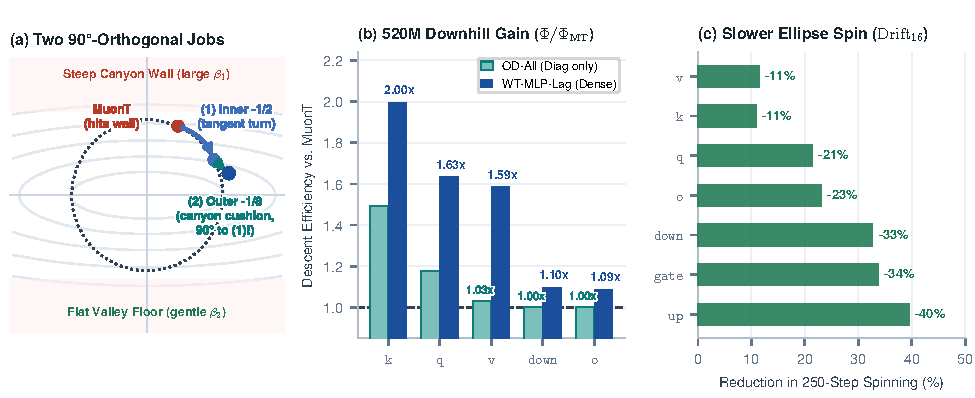
\includegraphics[width=\textwidth]{fig5_canyon_payoff.pdf}
  \caption{\textbf{Why the rotated update system wins---locally in steep canyons and globally across 250+ steps.}
  \textbf{(a)} Inner $L = B^{-1/2}$ and outer $\hat{L} = \unitrms(B^{-1/8})$ perform $90^\circ$-orthogonal jobs: \textbf{(1)}~inner $L$ rotates \emph{tangentially along the unit circle} to point away from loud error spikes toward true input--error correlation, while \textbf{(2)}~outer $\hat{L}$ reshapes step lengths \emph{perpendicular to the circle}, shrinking steps into steep canyon walls ($\beta_1$) and lengthening steps along gentle valley floors ($\beta_2$).
  \textbf{(b)} At \texttt{520M} ($\dm=1{,}024$), dense \mname{WT-MLP-Lag} boosts net downhill progress per unit canyon curvature ($\Phi_{B,C}$) by $1.59\times\text{--}2.00\times$ on \texttt{v, q, k} and $1.09\times\text{--}1.10\times$ on residual \texttt{o, down}, whereas diagonal \mname{OD-All} flatlines at $1.00\times$ on residual writers.
  \textbf{(c)} Over 250 training steps, avoiding canyon-wall overshoots slows backward error-oval spinning ($\mathrm{Drift}_{16}$) by $11\%\text{--}40\%$ across all seven layer types, allowing 20-step Nesterov momentum to accumulate cleanly.}
  \label{fig:canyon}
\end{figure}

\subsection{Reason 1: Inner \texorpdfstring{$L = B^{-1/2}$}{L = B\^{}(-1/2)} Selects Axes by Correlation, Not Error Loudness}
\label{sec:reason_cca}

Look at what an unnormalized momentum entry actually measures: if input activations have already been whitened ($\tilde{x} = C^{-1/2} x$, unit variance), then $Z_0 \approx \E[\delta \tilde{x}^{\Tr}]$.
Along any output error axis $q_i$ with RMS loudness $\sqrt{\beta_i}$ (so $\delta_i = \sqrt{\beta_i}\,\tilde{\delta}_i$ where $\tilde{\delta}_i$ has unit variance), row $i$ of $Z_0$ equals:
\begin{equation}
  q_i^{\Tr} Z_0 \;=\; \underbrace{\sqrt{\beta_i}}_{\text{Error Loudness}} \times \underbrace{\E\!\left[\tilde{\delta}_i\,\tilde{x}^{\Tr}\right]}_{\text{True Input--Error Correlation}}.
  \label{eq:loudness_vs_corr}
\end{equation}
Imagine two output directions:
\begin{itemize}[leftmargin=1.5em, itemsep=1.5pt, topsep=2pt]
  \item \textbf{Direction A (noisy canyon wall):} Error bounces wildly between $+50$ and $-50$ ($\sqrt{\beta_A} = 50$), with only weak $0.10$ correlation to the input ($\text{row length} = 50 \times 0.10 = \mathbf{5.0}$).
  \item \textbf{Direction B (clean learning feature):} Error steadily signals $+1$ ($\sqrt{\beta_B} = 1$), with strong $0.90$ correlation to the input ($\text{row length} = 1 \times 0.90 = \mathbf{0.9}$).
\end{itemize}
Without $L$, \mname{MuonT} thinks Direction~A is $5.5\times$ more important than Direction~B purely because it is noisy!
Multiplying on the left by $L = B^{-1/2}$ divides row $i$ by $\sqrt{\beta_i}$, cancelling out the loudness factor in \eqref{eq:loudness_vs_corr} and leaving \textbf{pure statistical correlation} $\E[\tilde{\delta}\tilde{x}^{\Tr}]$ (known in statistics as \emph{Canonical Correlation Analysis}).
In our \texttt{130M} checkpoints, this improves alignment between the orthogonalized update and each mode's true gradient across \textbf{$69\%\text{--}82\%$ of all quieter (\texttt{bot80}) output directions}.

\subsection{Reason 2: Outer \texorpdfstring{$\hat{L} = \unitrms(B^{-1/8})$}{L\_hat = unitRMS(B\^{}(-1/8))} Cushions Steep Canyon Walls (\texorpdfstring{$90^\circ$}{90 deg} to Inner \texorpdfstring{$L$}{L})}
\label{sec:reason_outer}

Why do we \emph{also} multiply by $\hat{L} = \unitrms(B^{-1/8})$ \emph{after} $\polar(\cdot)$?
Imagine hiking down a narrow canyon (\Cref{fig:canyon}a): north--south is a $16\times$ steeper rocky wall ($\beta_1 = 16$), while east--west is a gentle valley floor ($\beta_2 = 1$).
Even if inner $L$ points your compass axes cleanly, $\polar(L Z_0)$ resets \textbf{every axis back to step length $1.0$}! Taking a full step of $1.0$ east \emph{and} a full step of $1.0$ north slams you straight into the canyon wall.

\begin{toybox}[How Outer $B^{-1/8}$ Cuts Canyon Shock by $29\%$ Without Changing Step Size]
Suppose after $\polar(L Z_0)$, an orthogonal update puts unit energy $(1,\, 1)$ into a steep wall ($\beta_1 = 16$) and a gentle floor ($\beta_2 = 1$). Its total squared norm is $1^2 + 1^2 = 2.0$, and its canyon-wall curvature shock is $\beta_1(1)^2 + \beta_2(1)^2 = 16 + 1 = \mathbf{17.0}$.

Now apply outer $\hat{L} = \unitrms(B^{-1/8})$:
\begin{enumerate}[leftmargin=1.5em, itemsep=1.5pt, topsep=2pt]
  \item Raw $-1/8$ weights: $16^{-1/8} = 0.7071$ (shrinks steep wall) and $1^{-1/8} = 1.000$ (keeps valley floor).
  \item Rescale by $\unitrms$ so average squared weight stays $1.0$: $\hat{\ell}_1 = \sqrt{2/3} \approx \mathbf{0.816}$, $\hat{\ell}_2 = 2/\sqrt{3} \approx \mathbf{1.155}$.
  \item \textbf{Check step norm:} $\hat{\ell}_1^2 + \hat{\ell}_2^2 = \frac{2}{3} + \frac{4}{3} = \mathbf{2.000}$ (\emph{zero step-size inflation!}).
  \item \textbf{Check canyon shock:} $16(\frac{2}{3}) + 1(\frac{4}{3}) = \mathbf{12.0}$ --- a \textbf{$29.4\%$ drop in steep-wall shock} at the exact same total step length!
\end{enumerate}
\end{toybox}

\paragraph{Why inner $L$ and outer $\hat{L}$ are $90^\circ$ perpendicular---never redundant.}
Look again at \Cref{fig:canyon}a: inner $L$ moves the update \emph{along the unit circle} of orthogonal matrices (changing angle while keeping singular values $=1$), whereas outer $\hat{L}$ stretches and compresses \emph{radially perpendicular to the circle} (changing singular values along $B$'s axes).
When we measure the angle between the inner update change $\Delta_{\mathrm{in}}$ and outer update change $\Delta_{\mathrm{out}}$ across all 160 $\dm$-wide matrices of our \texttt{130M} Transformer, their cosine is $[-0.002, +0.027]$---literally \textbf{$88.4^\circ\text{--}90.1^\circ$ perpendicular}! Dropping inner $L$ in our ablations (\mname{Abl-OuterDense}) immediately loses one-third of the validation gain.

\paragraph{Why a gentle $-1/8$ outside instead of $-1/4$ (\mname{GO-MUON}) or $-1/2$?}
If shrinking steep walls is good, why not use a stronger $-1/4$ or $-1/2$ exponent outside $\polar(\cdot)$, as \mname{GO-MUON}~\citep{che2026gomuon} does?
Because in stochastic deep learning, tiny eigenvalues $\beta_{\min} \approx 10^{-3}$ of $B_t$ are not just ``flat valley floors''---they are dominated by \textbf{random minibatch label noise}!
Compare how much each outer exponent amplifies a tiny noisy mode $\beta_{\min} = 10^{-3}$:
\begin{equation}
  (10^{-3})^{-1/8} \approx \mathbf{2.4\times}\text{ (ours)},
  \quad
  (10^{-3})^{-1/4} \approx \mathbf{5.6\times}\text{ (\mname{GO-MUON})},
  \quad
  (10^{-3})^{-1/2} \approx \mathbf{31.6\times}.
  \label{eq:noise_amp}
\end{equation}
That single line explains \mname{GO-MUON}'s dramatic curve in the main paper: $-1/4$ plunges rapidly during the first $20$ steps while big initial gradients dominate, then amplifies tail cotangent noise by $1.25\times\text{--}1.29\times$ and crashes $+0.03$ nats \emph{worse} than plain \mname{Muon} after step $200$.
Our decoupled $(-1/2\text{ inside},\, -1/8\text{ outside})$ split gets full fair-voting rotation inside $\polar(\cdot)$ while keeping post-polar noise calm---boosting net downhill efficiency $\Phi_{B,C}$ across every projection at both \texttt{130M} and \texttt{520M} (\Cref{fig:canyon}b).

\subsection{Reason 3: Calmer Steps Stop Error Ovals from Spinning, Helping Momentum Add Up}
\label{sec:reason_drift}

Finally, optimization is a movie, not a single snapshot.
\mname{Muon} accumulates a 20-step exponential moving average of gradients ($M_t = 0.95 M_{t-1} + G_t$).
Imagine adding 20 arrows together:
\begin{itemize}[leftmargin=1.5em, itemsep=1.5pt, topsep=2pt]
  \item Under \mname{MuonT}, unpreconditioned output steps repeatedly overshoot steep cotangent walls, causing upper-layer representations and backward error ovals $B_t$ to lurch and spin rapidly. Arrows from 10 steps ago point in stale directions and partially cancel today's gradient.
  \item Under \mname{WT-MLP-Lag}, cushioning steep output modes keeps layer outputs changing smoothly. Across all seven layer types (\Cref{fig:canyon}c), 250-step error-oval spinning ($\mathrm{Drift}_{16}$) slows down by \textbf{$11\%\text{--}40\%$} (for example, $33\%$ slower on \texttt{down} and $34\%\text{--}40\%$ slower on \texttt{gate, up}), allowing 20-step Nesterov momentum to add up constructively step after step!
\end{itemize}

% ===========================================================================
\section{One-Page Cheat Sheet: How Every Piece of WT-MLP-Lag Fits Together}
\label{sec:cheatsheet}
% ===========================================================================

When you return to the main paper (\texttt{paper\_v3/main.pdf}), the entire \mname{WT-MLP-Lag} algorithm reduces to one master update equation:
\begin{equation}
  D_{p,t} \;=\;
  \underbrace{\hat{L}_{p,t-1}}_{\substack{\text{Outer }-1/8\\\text{canyon cushion}}}
  \;\Nten\!\Bigl(
    \underbrace{L_{p,t-1}}_{\substack{\text{Inner }-1/2\\\text{fair-vote rotation}}}
    \,U_{p,t}\,
    \underbrace{R_{p,t}}_{\substack{\text{Input }-1/2\\\text{(\mname{MuonT})}}}
  \Bigr)\,
  \underbrace{\hat{R}_{p,t}}_{\substack{\text{Input }-1/8\\\text{(\mname{MuonT})}}}.
  \label{eq:master_cheat}
\end{equation}
\Cref{tab:cheatsheet} connects every design choice in \eqref{eq:master_cheat} directly to the visual intuition we built in \Cref{sec:primer,sec:rotation_meaning,sec:hijacking,sec:why_better}.

\begin{table}[ht]
  \centering
  \caption{\textbf{Complete Logic Map from Geometric Intuition to \mname{WT-MLP-Lag}'s Engineering Design.}}
  \label{tab:cheatsheet}
  \vspace{2pt}
  \footnotesize
  \renewcommand{\arraystretch}{1.26}
  \begin{tabular}{@{}>{\raggedright\arraybackslash}p{0.25\textwidth}>{\raggedright\arraybackslash}p{0.36\textwidth}>{\raggedright\arraybackslash}p{0.33\textwidth}@{}}
    \toprule
    \textbf{Design Choice in \mname{WT-MLP-Lag}} & \textbf{Visual / Geometric Reason} & \textbf{What Breaks If You Remove It?} \\
    \midrule
    \textbf{Keep dense input whitening $(R_t, \hat{R}_t)$ everywhere} & Even after RMSNorm, forward token activations cluster along low-rank directions (and post-SwiGLU \texttt{in:down} neurons fire together from shared inputs). & Dropping input whitening (\mname{Abl-OutOnly}) or diagonalizing \texttt{in:down} (\mname{WT-Sym-Lag}) degrades validation loss sharply. \\
    \textbf{Dense output roots $(L, \hat{L})$ at hidden width $\dm$ (\texttt{q, k, v, o, down})} & Residual mixing stirs all $\dm$ neurons together ($\mathrm{IPR} \approx 3.01$), tilting $>99\%$ of \texttt{o, down}'s error oval off-diagonal (\Cref{fig:tilted}b,c). & Diagonal \mname{OD-All} sees uniform diagonals ($B_{ii} \approx 1$), rotating \texttt{o, down} by only $4^\circ$ and losing its gain at \texttt{520M}. \\
    \textbf{1D diagonal output roots at expanded width $\dff = 4\dm$ (\texttt{gate, up})} & Elementwise SwiGLU gating scrambles cross-neuron backward correlations to zero ($\rho_{\mathrm{rms}} \approx 0.005$), leaving an axis-aligned oval (\Cref{fig:tilted}a). & Dense $O(\dff^3)$ roots (\mname{DT-All}) waste $96.2\%$ of output eigendecomposition FLOPs on sampling noise; dropping them (\mname{Abl-No2048}) loses $>50\%$ of gain. \\
    \textbf{Inner exponent $-1/2$ inside $\Nten$} & Prevents loud error channels from hijacking the $90^\circ$ polar vote (\Cref{fig:hijacking}) and wakes up quiet singular values inside 10-step $\Nten$. & Outer-only preconditioning (\mname{Abl-OuterDense}) leaves $30\%\text{--}68\%$ basis hijacking intact and forfeits $\sim 1/3$ of the loss gain. \\
    \textbf{Unit-RMS outer exponent $-1/8$ outside $\Nten$} & Acts at $90^\circ$ to inner $L$ (\Cref{fig:canyon}a) to shrink steps into steep canyon walls without inflating global step norm ($\|D\|_F$ ratio $0.985$). & Steep $-1/4$ outer roots with norm grafting (\mname{GO-MUON}) blow up noisy tail modes ($5.6\times$ vs.\ $2.4\times$) and diverge above \mname{Muon} after step 200. \\
    \textbf{1-step async lag ($\tau = 1$) on background stream} & Backward error ovals spin $10\times$ faster than inputs (triggering $22$ exact \texttt{eigh}/step) and finish only at the end of backward, but EMA averages $\sim 16$ steps. & Synchronous \mname{WT-MLP} stalls the step boundary ($+11.3\%$ vs.\ $+5.3\%$ overhead) for virtually identical validation loss. \\
    \bottomrule
  \end{tabular}
\end{table}

\begin{keyfinding}[One-Sentence Summary of the Entire Theory]
In \mname{Muon}, throwing away singular values means \textbf{your choice of perpendicular axes IS your optimizer}: output normalization rescues those axes from being hijacked by loud backward error spikes (inner $-1/2$), gently cushions steps into steep canyon walls (outer $-1/8$), uses full rotations only where residual mixing tilts the error oval ($\dm$) and cheap per-neuron scaling where SwiGLU aligns it ($\dff$), and thereby calms the network's error subspaces so momentum flows steadily downhill.
\end{keyfinding}

\bibliographystyle{plainnat}
\bibliography{refs}

\end{document}
